
\begin{figure*}[t]
    \centering
    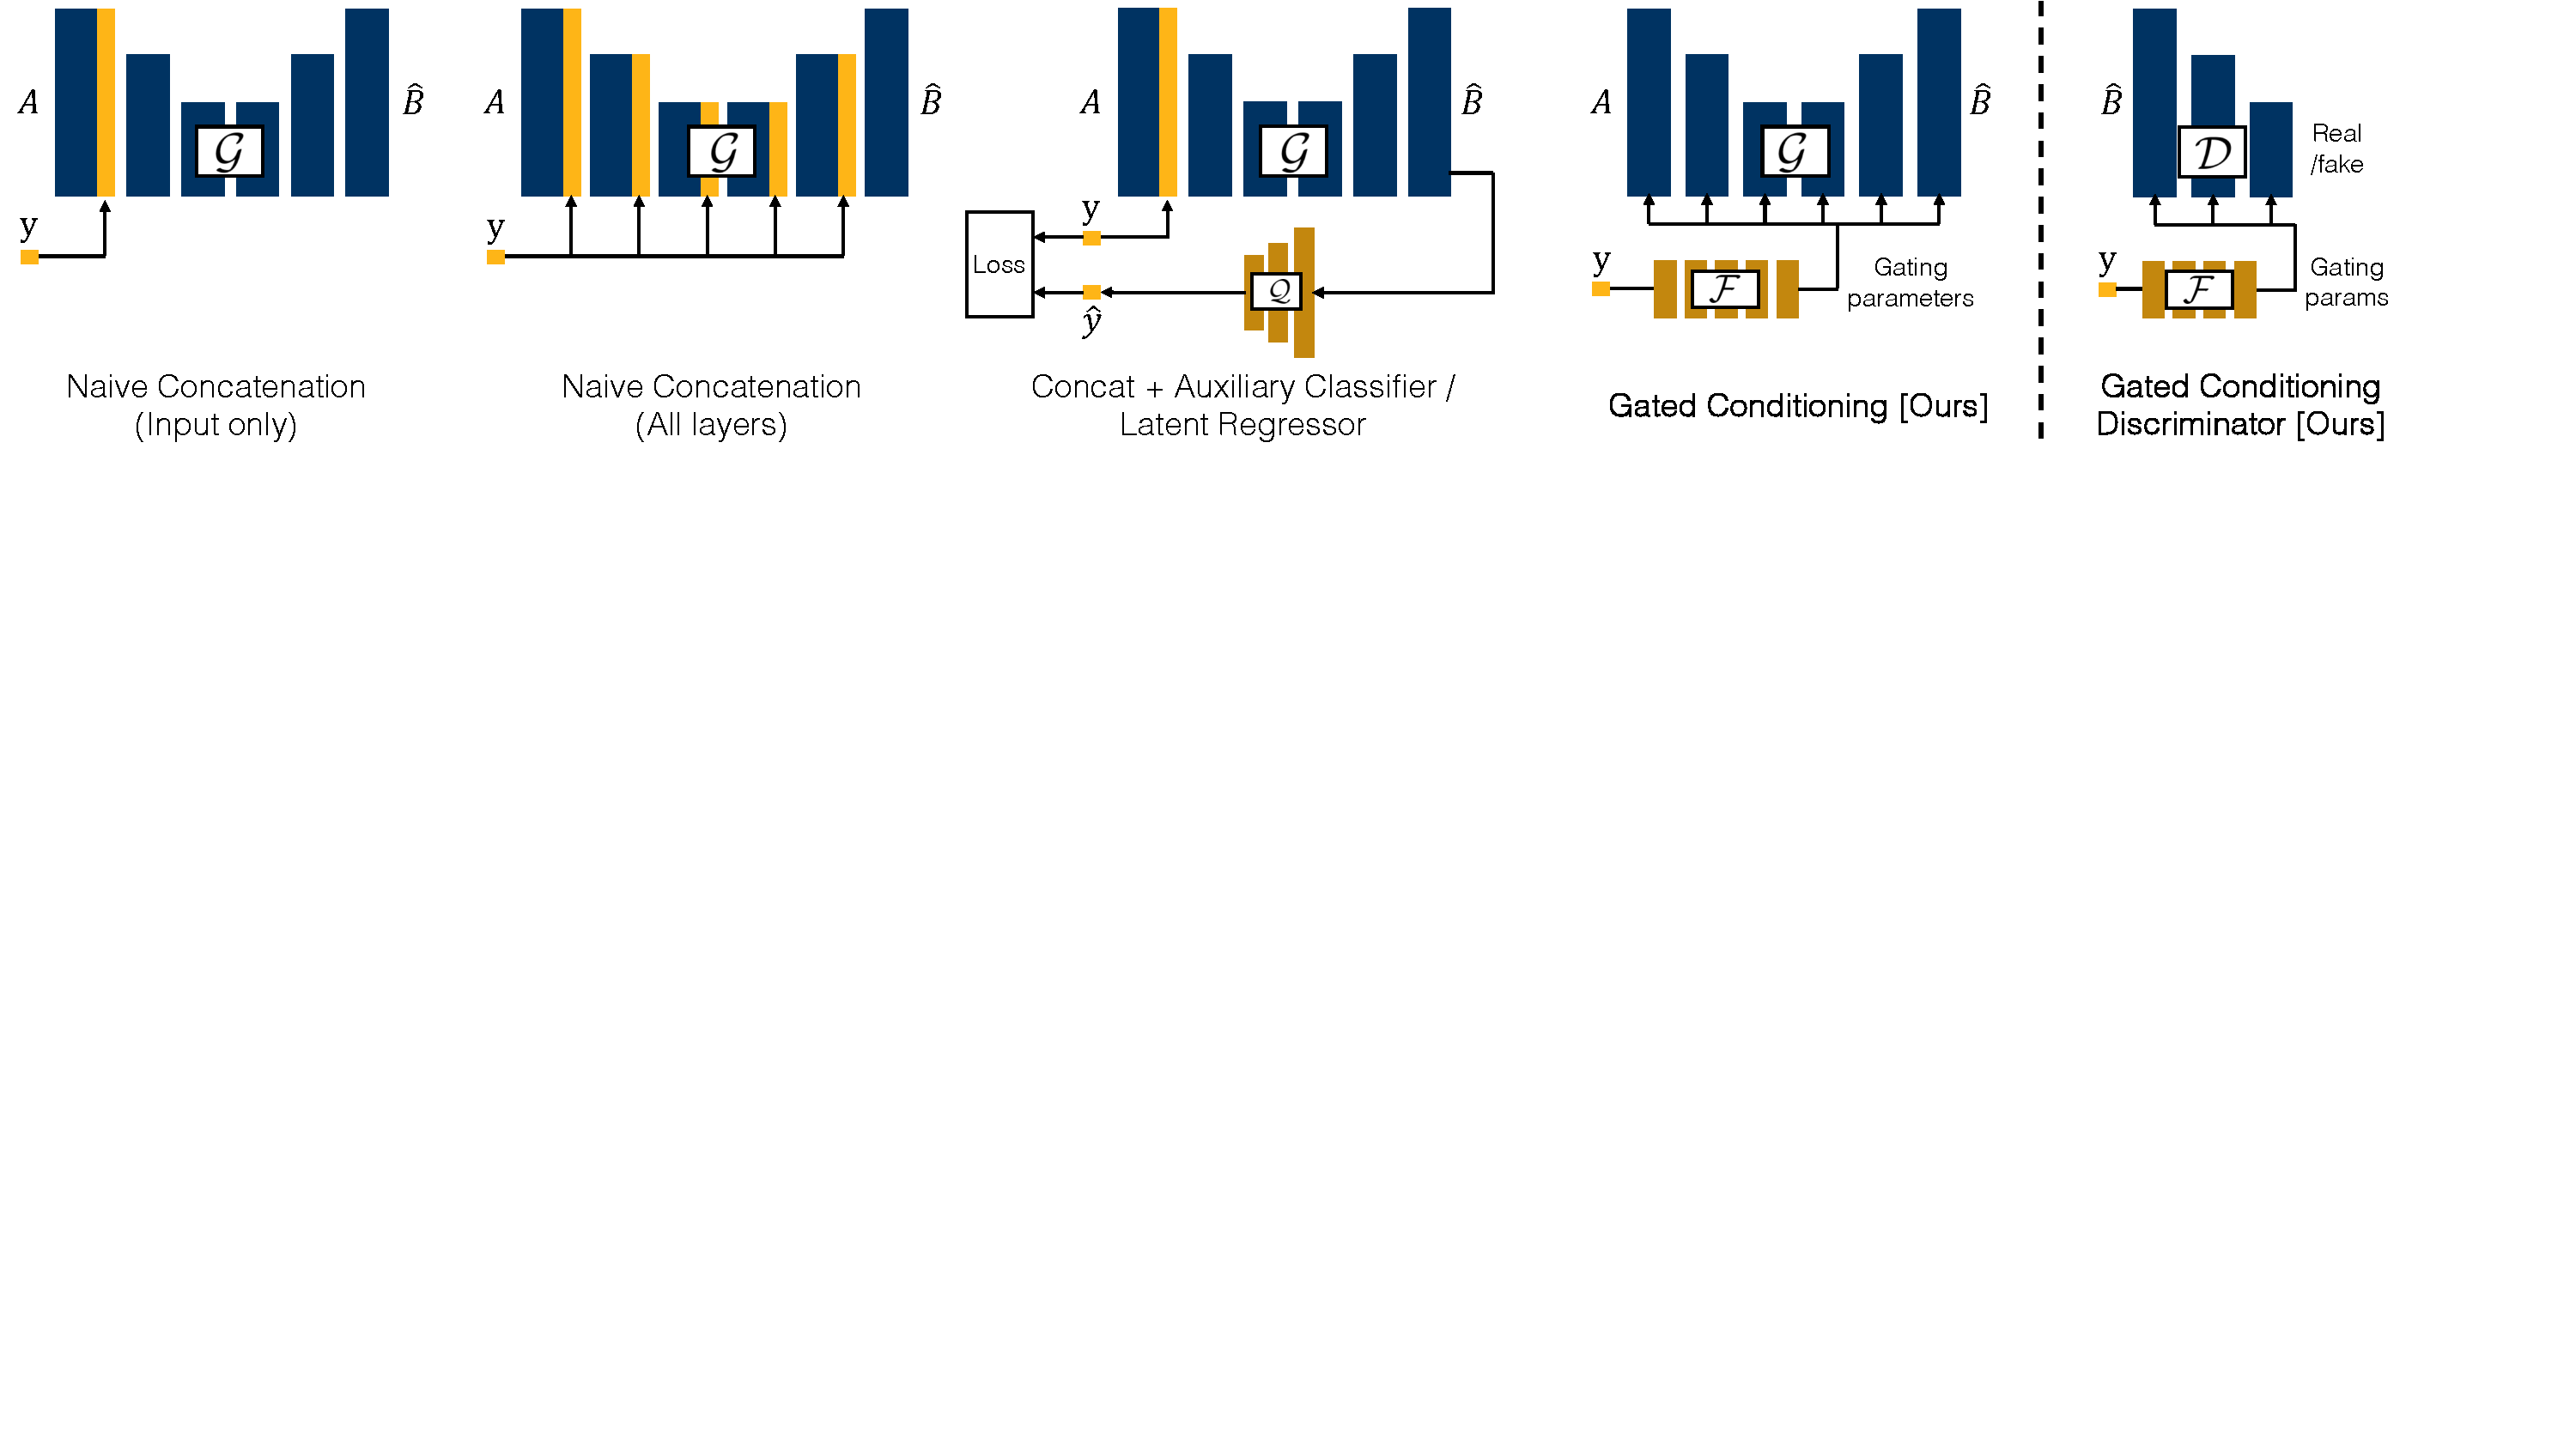
\includegraphics[width=\linewidth]{paper_images/arch_inject2.pdf}
    \caption{{\bf Conditioning injection variants.}
    The conditioner can be naively incorporated in a generator through simple concatenation in {\bf (left)} the input layer only or {\bf (mid-left)} in all layers. {\bf (mid)} The network can be further encouraged to use the conditioning through a learned network, using either a classification objective for categorical conditioning~\cite{odena2016conditional,chen2016infogan} or a regression objective for continuous conditioning. {\bf (Mid-right)} We train a network on the conditioner to predict parameters which guide softly-gated units in the main network. {\bf (Right)} These conditioning options can be correspondingly applied to a discriminator. We propose using soft-gating on the discriminator as well.\label{fig:arch-inj}
    \vspace{-2mm}
    }
    \vspace{-2mm}
\end{figure*}

\section{Introduction}
Generative methods have made huge strides in the last few years, driven by the success of models such as Generative Adversarial Networks (GANs)~\cite{goodfellow2014generative} and Variational Autoencoders (VAEs)~\cite{kingma2013auto}.
% These methods can generate impressive results, but
One major challenge is that quality can degrade when the diversity of training data increases.
% (e.g., number of object/scene classes).
A common practice in conditional image conditional generation is to train different models for different tasks~\cite{isola2016image2image,karras2017progressive,zhu2017toward,zhu2017unpaired,wang2017high,wang2018video}, meaning that parameters scale linearly with the number of tasks.
%However their proposed method still involved training multiple generators.
% A study performed in \cite{ghosh2017multi,metz2017unrolledGAN} demonstrated that even in a simple 1D \& 2D Mixture of Gaussians settings, state-of-the-art GAN techniques were not able to generate samples from all the components of the mixture. 
This presents an intriguing opportunity -- ideally, a single network can solve multiple tasks. Such a network would have the flexibility to share operations applicable across tasks, while dedicating resources responsible for task-specific operations.
% An ideal scenario in such settings would involve a single network which could share parts responsible for similar operations across classes while unsharing the discrete parts of the network which are responsible for class specific operations.

% Such a scenario was analyzed in the realm of
In image classification, Veit et al.~\cite{veit2016residual} show, through lesion experiments, that a Residual Network~\cite{he2016deep} implicitly allows information flow through multiple paths. Follow-up work~\cite{veit2018adaptive} aims to explicitly specialize different paths for different classes~\cite{veit2018adaptive}.
% In image classification, Veit et al.~\cite{veit2016residual} perform incision experiments on a pretrained ResNet architecture~\cite{he2016deep}, demonstrating that certain paths in the network play a more important role for certain classes.
%inferring that ResNets behave like an ensemble of several partially disjoint networks for image classification. 
In this paper, we analyze the implications of this observation in a generative modeling scenario. 
We analyze GANs on a 1D Mixture of Gaussians distribution, as used in~\cite{ghosh2017multi}, and discover that removal of blocks corresponds to the disappearance of certain modes in the generated distribution.

Motivated by this, we introduce a simple {\em soft-gating} mechanism, where a hypernetwork on the conditioning input determines which blocks of a ResNet to use.
% to use for that particular conditioning.
We explore and analyze different types of gating, including {\em blockwise} and {\em channelwise} gating, each with multiplicative and affine variations, as well as related methods for incorporating conditioning information. We draw connections to AdaIn~\cite{huang2017arbitrary,huang2018multimodal} and InfoGAN~\cite{chen2016infogan}. We show that channelwise multiplicative gating performs best for our task, and better results can be obtained by gating not only the generator, but also the discriminator.

To evaluate our approach, we introduce a new task of generating multiclass images from rough outline scribbles, where class ambiguities are especially challenging. Fig.~\ref{fig:teaser} (top-left) shows one such example, where the same circular outline yields different outputs, conditioned on ten different classes.
In the unsupervised InfoGAN~\cite{chen2016infogan} setting, where classes are not known apriori, conditioning is in the form of a random vector. 
While this scenario was previously shown to produce limited texture variation~\cite{ghosh2017multi} for challenging datasets using naive concatenation-based conditioning, our method is able to produce diverse generations, as shown in Fig.~\ref{fig:teaser} (top right).
In addition, we evaluate our approach on {\em multitask image-to-image translation}. 
In its original setting \cite{isola2016image2image}, individual models were used for each translation tasks. 
Our gating mechanism enables good performance of a single network on multiple tasks by activating appropriate task-specific blocks and channels (Fig.~\ref{fig:teaser} bottom).

%whereby the rough scribbles divulge almost no information about the class.



%%The technique presented a scenario in which we could generate multiple modes for a single dataset but it could further be used for generating multiple modes from a dataset consisting of multiple classes and the hypernetwork could choose the blocks needed for a particular class. 




%%Furthermore we perform a systematic analysis of all meaningful gating mechanisms and other forms of conditioning in the setting of a image conditioned generative model. This paper also finds that gating also enables the discriminator to provide better class conditioned gradients back to the generator for high quality generations.


% Generative methods have made huge strides in the last few years driven by the success of Variational Autoencoders (VAEs)~\cite{kingma2013auto} and Generative Adversarial Networks (GANs)~\cite{goodfellow2014generative}. 
% While these methods can generate impressive results, one major challenge is that quality degrades quickly when the diversity of training data (e.g., number of object/scene classes) increases, especially when the manifold of the multi-class distribution of images drawn from the ground truth distribution is not continuous. \ow{um... I don't really get this previous sentence}

% We propose a solution to generate multi-class images using a form of class conditioning that outperforms prior class conditioned GANs while requiring significantly fewer parameters than using a single GAN per-class. 
% To do this, we take advantage of the fact that different classes will share similar visual features, and propose an architecture wherein a fully-residual GAN generator and discriminator, is combined with a second ``gating'' network, which determines how the network is conditioned on the input class.

% We compare various forms of gating, such as concatenating one-hot class information, auxillary classification, \todo{...}.

% We evaluate our gating approach on a number of applications \todo{...}
% \ow{discuss evaluation and findings}

In summary, our contributions are:
\vspace{-2mm}
% \setlength\itemsep{0px}
% \begin{itemize}
\begin{itemize}[noitemsep]
% \itemsep0em 
% \item An in-depth analysis of the role of gating networks in generative modeling.
% \item an in-depth analysis of the role of gating networks in generative modeling
\item a systematic analysis of variants for injecting conditioning into a generative model
\item a novel \textit{soft-gating} mechanism, which enables effective incorporation of a conditioning vector in multiclass (class-conditioned), multimodal (latent code-conditioned), and multitask (task-conditioned) image-to-image translation settings
% \item A novel architecture using a soft-gating hypernetwork that can generate diverse, multiclass results both when classes are known apriori, or are derived from the data in an unsupervised fashion.
% (similar to InfoGAN~\cite{chen2016infogan}).
%\item Incision experiments on a trained Residual Generator based GAN on the 1D Mixture of Gaussians to show certain blocks correspond to certain modes in the generated distribution.
%\item Introduction of the Gated Residual Blocks and the Hypernetwork to predict the corresponding alphas on the Generator and Discriminator.
\item introduction of a challenging outline$\rightarrow$image dataset
% of generating realistic images from a rough outline.
\end{itemize}

\vspace{-1mm}